% ============================================================
%  N.3.1  Full-Sized Architecture: Fusion Mode Comparison
% ============================================================
\subsection{Full-Sized Architecture: Fusion Mode Comparison (Scenario~A)}
\label{sec:fusion-full-sized}

\subsubsection{Motivation}

The case studies presented in Sections~\ref{sec:eyeriss-cs1}
through~\ref{sec:eyeriss-cs5} focused on how individual
architectural parameters, such as register sizes and PE aspect
ratios, interact with the fusion mapping.
This section shifts perspective and answers the question:
\emph{does layer fusion actually improve the end-to-end efficiency
of a DNN accelerator, and under what conditions?}

To answer this, we define three execution modes on the same
architecture instance, which is sized to support full fusion of the
entire workload (Scenario~A):
\begin{enumerate}
  \item \textbf{Full fusion.}
        All convolutional layers are fused into a single mapping.
        Intermediate activations are kept entirely on chip, reducing
        DRAM traffic to the network's input and final output only.
  \item \textbf{Partial fusion (sum).}
        Consecutive layer groups are fused independently.
        The total cost is the sum of all fused evaluations.
        DRAM traffic is reduced for each group, but intermediate
        activations between non-fused layers still traverse DRAM.
  \item \textbf{Single-layer (sum).}
        Each layer is mapped in isolation, and the total cost is
        the sum of all individual layer evaluations.
        Every intermediate activation is written to and read back
        from DRAM.
\end{enumerate}

The architecture used for each workload is the same full-fusion
configuration determined by the PE and memory sizing studies done
(Table~\ref{tab:fusion-auto-configs}).
Running partial and single-layer modes on a full-fusion-sized
architecture provides a fair comparison because all three modes
share identical hardware; only the inter-layer mapping
strategy differs.

\begin{table}[htbp]
  \centering
  \caption{Architecture configurations used for Scenario~A
    (full-fusion-sized).
    Memory sizes refer to the DepFiN feature-memory (fmem) and
    weight-memory (wmem), or the Eyeriss GlobalBuffer (GB) and
    per-PE weight register (WReg).}
  \label{tab:fusion-auto-configs}
  \begin{tabular}{ll rr rr}
    \toprule
    & & \multicolumn{2}{c}{DepFiN} & \multicolumn{2}{c}{Eyeriss} \\
    \cmidrule(lr){3-4} \cmidrule(lr){5-6}
    Workload & PEs
      & fmem & wmem
      & GB & WReg \\
    \midrule
    FSRCNN   & $16 \times 128$ / $128 \times 16$
      & 576\,KB  & 19\,KB
      & 128\,KB  & 384 \\
    MC-CNN   & $8 \times 256$\, / $256 \times 8$
      & 522\,KB  & 32\,KB
      & 128\,KB  & 384 \\
    VGG16    & $16 \times 128$ / $512 \times 32$
      & 568\,KB  & 14\,366\,KB
      & 128\,KB  & 1\,200 \\
    ResNet18 & $16 \times 128$ / $512 \times 32$
      & 266\,KB  & 10\,738\,KB
      & 128\,KB  & 902 \\
    \bottomrule
  \end{tabular}
\end{table}

The following analysis is organized around three metrics, each
normalized to the full-fusion value, and concludes with the
DRAM traffic reduction and a summary of the key findings.

\subsubsection{Results}

% ── Energy ──────────────────────────────────────────────────
\paragraph{Energy (Figure~\ref{fig:fusion-energy-norm}).}
Whether full fusion saves or wastes energy depends critically on
the balance between two opposing effects: the elimination of DRAM
traffic for intermediate activations and the increased per-access
cost of the enlarged on-chip memories required to support fusion.
At 160\,pJ\,/\,byte for DRAM
(Section~\ref{sec:energy-model}), the outcome is
workload-dependent and architecture-dependent.

On \textbf{DepFiN}, full fusion is the most energy-efficient mode
for the two activation-dominant workloads.
FSRCNN in single-layer mode consumes $4.38\times$ the full-fusion
energy, and MC-CNN consumes $1.73\times$.
The explanation is that these workloads generate massive
intermediate-activation volumes (Section~\ref{sec:dram-traffic}),
and the DRAM energy eliminated by fusion
vastly exceeds the extra on-chip cost (576\,KB for FSRCNN, 522\,KB for MC-CNN).
Partial fusion also benefits, sitting at $1.47\times$ full for
FSRCNN and $1.43\times$ for MC-CNN.

For the weight-dominant workloads on DepFiN, the picture reverses.
VGG16 single-layer execution costs only $7.4\%$ of the
full-fusion energy, and ResNet18 costs $17.3\%$.
Fusion requires a weight memory of 14\,366\,KB (VGG16) or
10\,738\,KB (ResNet18) to hold all weights on chip
simultaneously.
Every weight access through these large memories incurs an
elevated per-access energy that compounds across billions of multiply accumulations (MACs).
Because the intermediate-activation volume is comparatively small,
the DRAM savings are insufficient to compensate.
Partial fusion partially mitigates this: its normalized energy is
$0.49$ for VGG16 and $0.75$ for ResNet18, confirming that fusing
only a few layers at a time requires less inflated memory.

On \textbf{Eyeriss}, full fusion is roughly energy-neutral for
FSRCNN (single\,$= 0.985\times$\,full), suggesting that the DRAM
savings and the register overhead nearly cancel.
For all other workloads, full fusion is again the most expensive
mode: MC-CNN single costs $45.0\%$ of full, VGG16 single costs
$5.9\%$, and ResNet18 single costs $12.6\%$.
The Eyeriss energy penalty is driven by the replicated register
architecture: with 16\,384~PEs for VGG16, the aggregate weight
register capacity is $1{,}200 \times 16{,}384 = 19.7$~million
bytes, each contributing to per-access energy.
Despite the high DRAM cost, the vast volume of on-chip accesses
through these large registers dominates the energy budget.
Partial fusion is consistently cheaper than full fusion on
Eyeriss, with normalized values of $0.66$ (FSRCNN), $0.65$
(MC-CNN), $0.39$ (VGG16), and $0.69$ (ResNet18).

\begin{figure}[htbp]
  \centering
  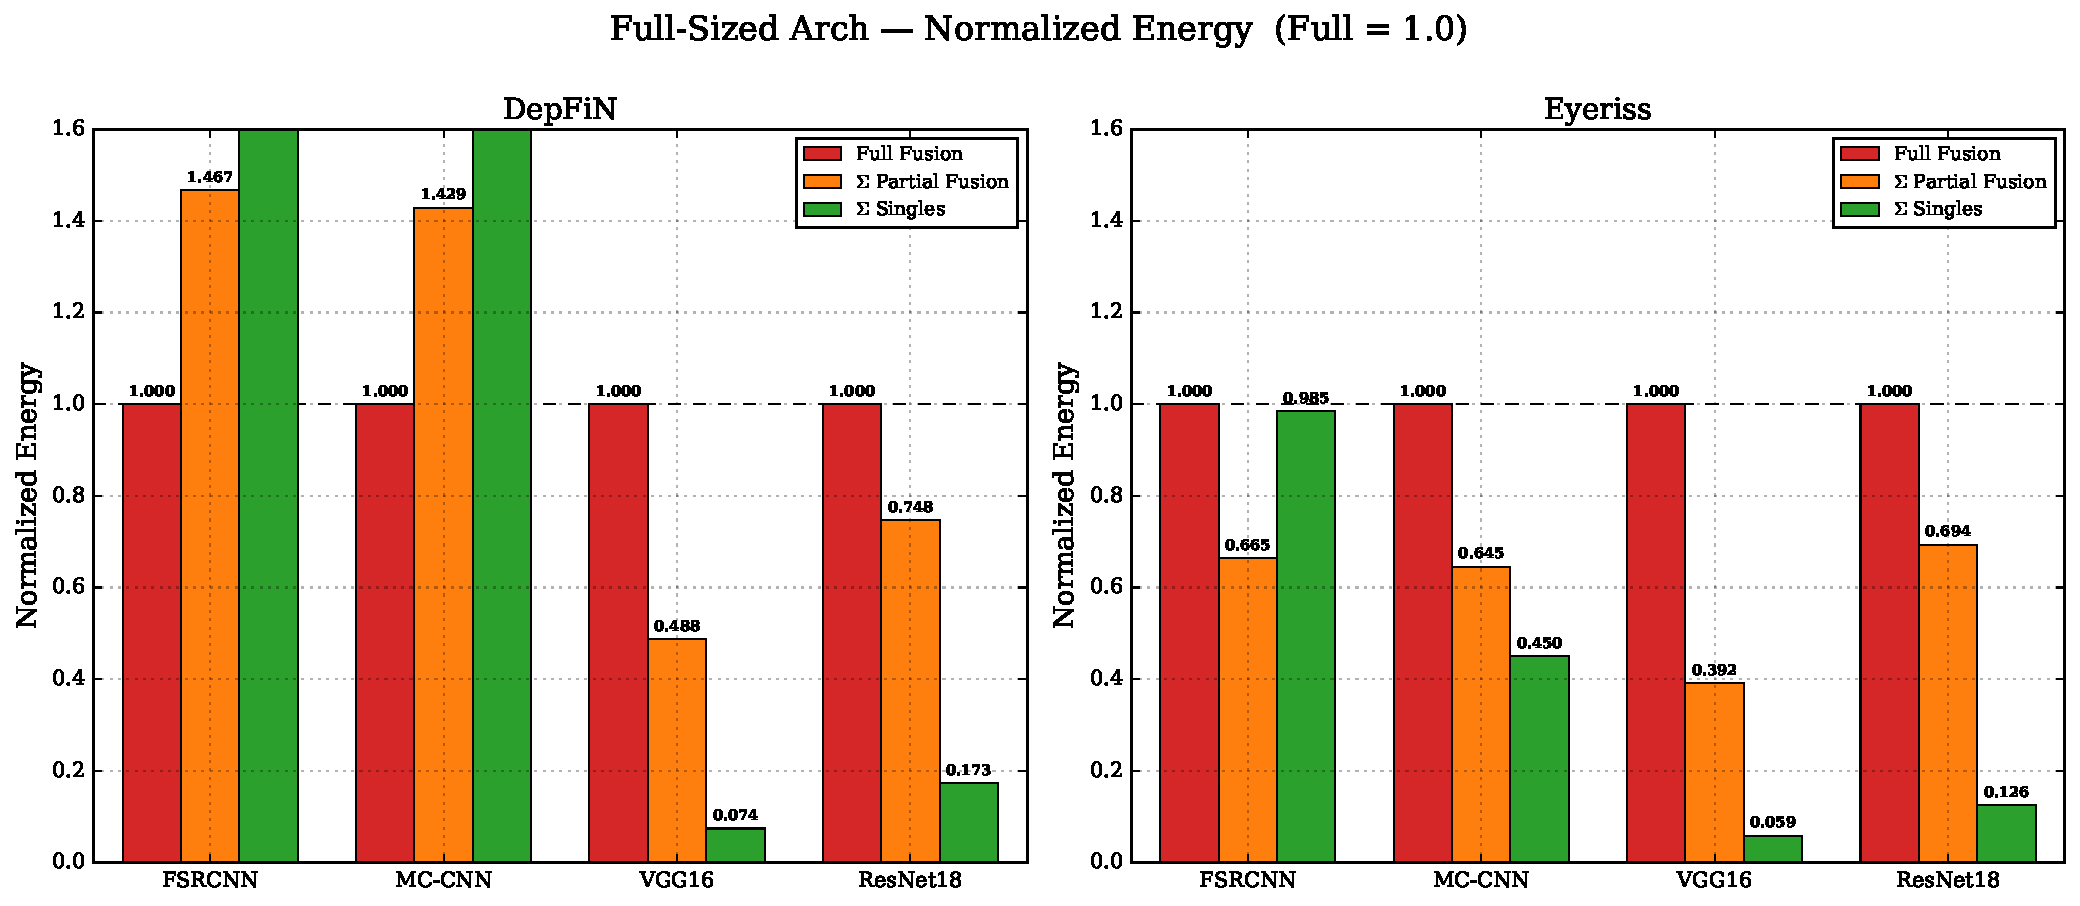
\includegraphics[width=0.95\textwidth]{plots/fusion_auto_energy_norm.pdf}
  \caption{Scenario~A: Normalized energy (Full~Fusion\,=\,1.0).
    Bars below 1.0 indicate lower energy than full fusion.
    Values annotated above each bar.}
  \label{fig:fusion-energy-norm}
\end{figure}

% ── Latency ─────────────────────────────────────────────────
\paragraph{Latency (Figure~\ref{fig:fusion-latency-norm}).}
Full fusion delivers latency benefits whose magnitude depends on the workload and architecture.

For the activation-dominant workloads, full fusion is clearly
faster on both architectures.
FSRCNN enjoys a $47.6\%$ latency saving on DepFiN and $45.6\%$
on Eyeriss, while MC-CNN saves $42.3\%$ on DepFiN and $15.7\%$
on Eyeriss (Figure~\ref{fig:fusion-latency-savings}).
These workloads have large intermediate-activation volumes
relative to their weight volumes, so eliminating the DRAM
round-trips for activations removes the dominant bottleneck from
the execution timeline.

For the weight-dominant workloads the behavior diverges across
architectures.
On Eyeriss, full fusion still reduces latency compared to the
single-layer sum: VGG16 saves $21.2\%$ and ResNet18 saves
$7.8\%$.
On DepFiN, however, full fusion is \emph{slower} than the
single-layer sum: VGG16 loses $11.3\%$ and ResNet18 loses
$30.3\%$.
Eyeriss avoids this penalty because its distributed per-PE
register architecture keeps each layer's weight factors local,
allowing to compute without a unique
shared memory contention point for all the layers, the weight memory.

Partial fusion tracks the full-fusion latency closely in most
cases: the ratio ranges from $0.87\times$ (ResNet18, DepFiN) to
$1.07\times$ (VGG16, Eyeriss), indicating that the latency
benefit of fusion is captured almost entirely by pairwise fusion,
with little additional gain from fusing all layers
simultaneously.

\begin{figure}[htbp]
  \centering
  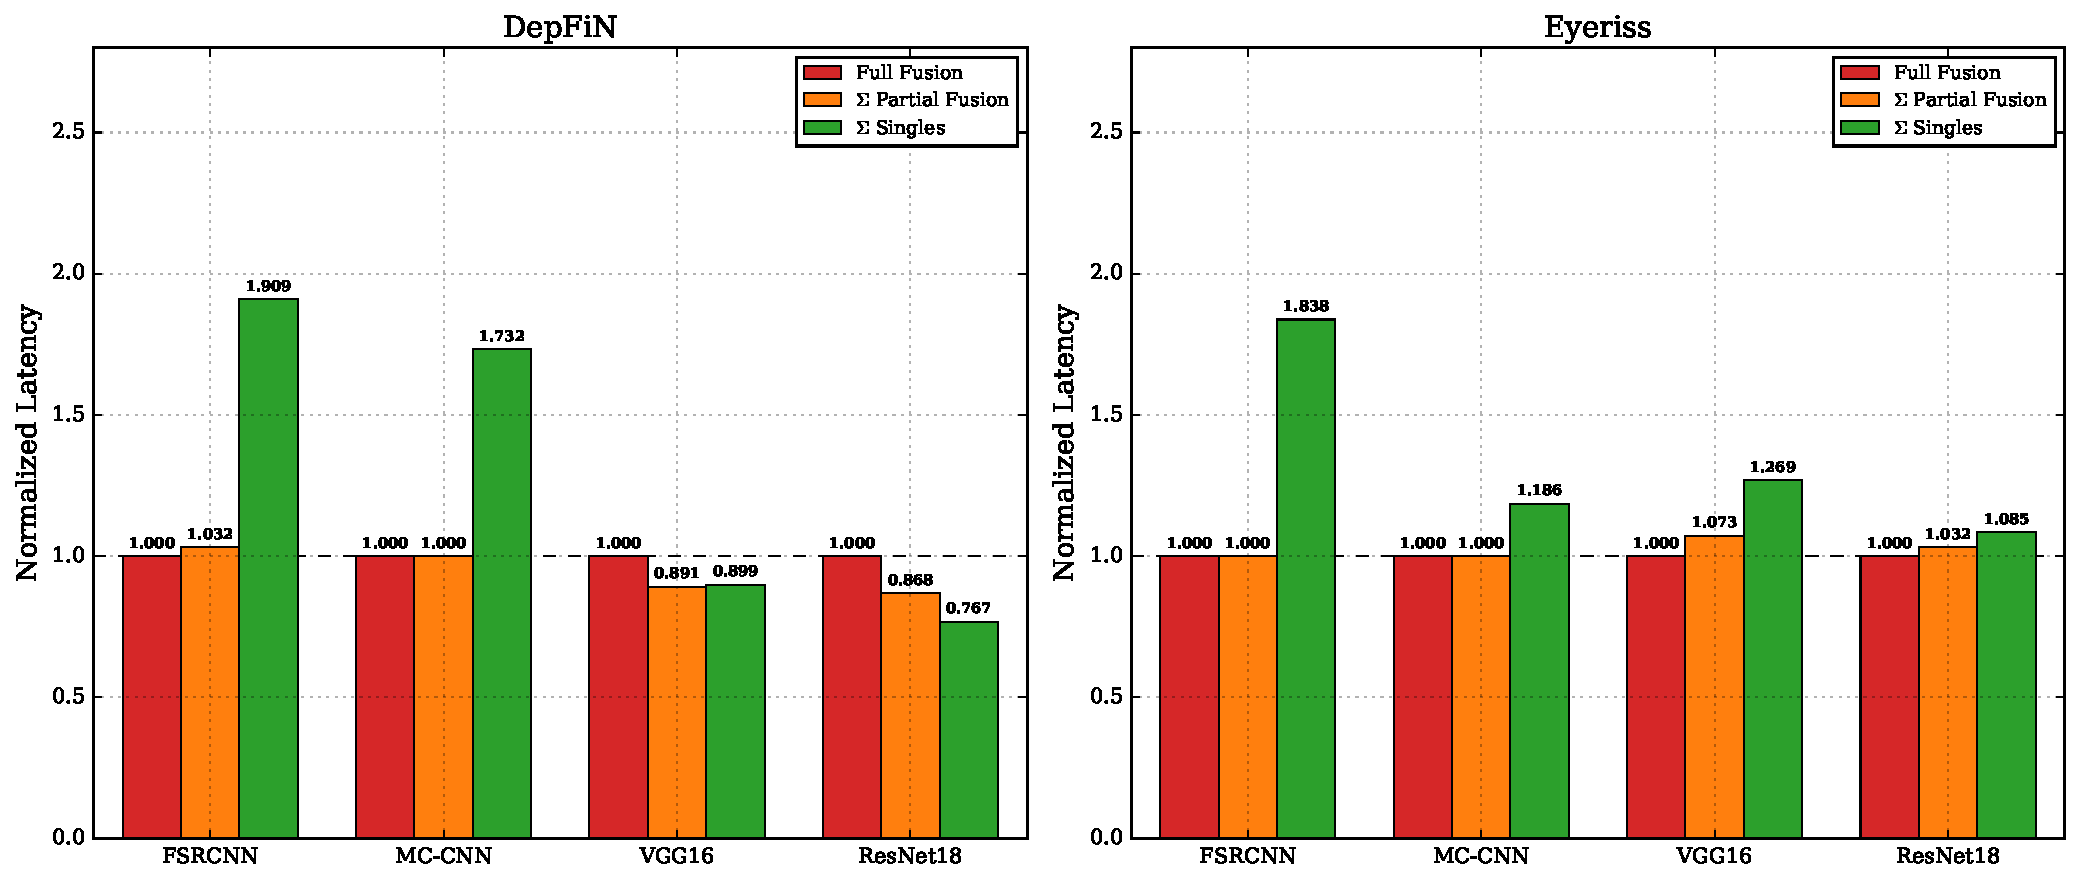
\includegraphics[width=0.95\textwidth]{plots/fusion_auto_latency_norm.pdf}
  \caption{Scenario~A: Normalized latency (Full~Fusion\,=\,1.0).
    Bars above 1.0 indicate longer latency than full fusion.}
  \label{fig:fusion-latency-norm}
\end{figure}

\begin{figure}[htbp]
  \centering
  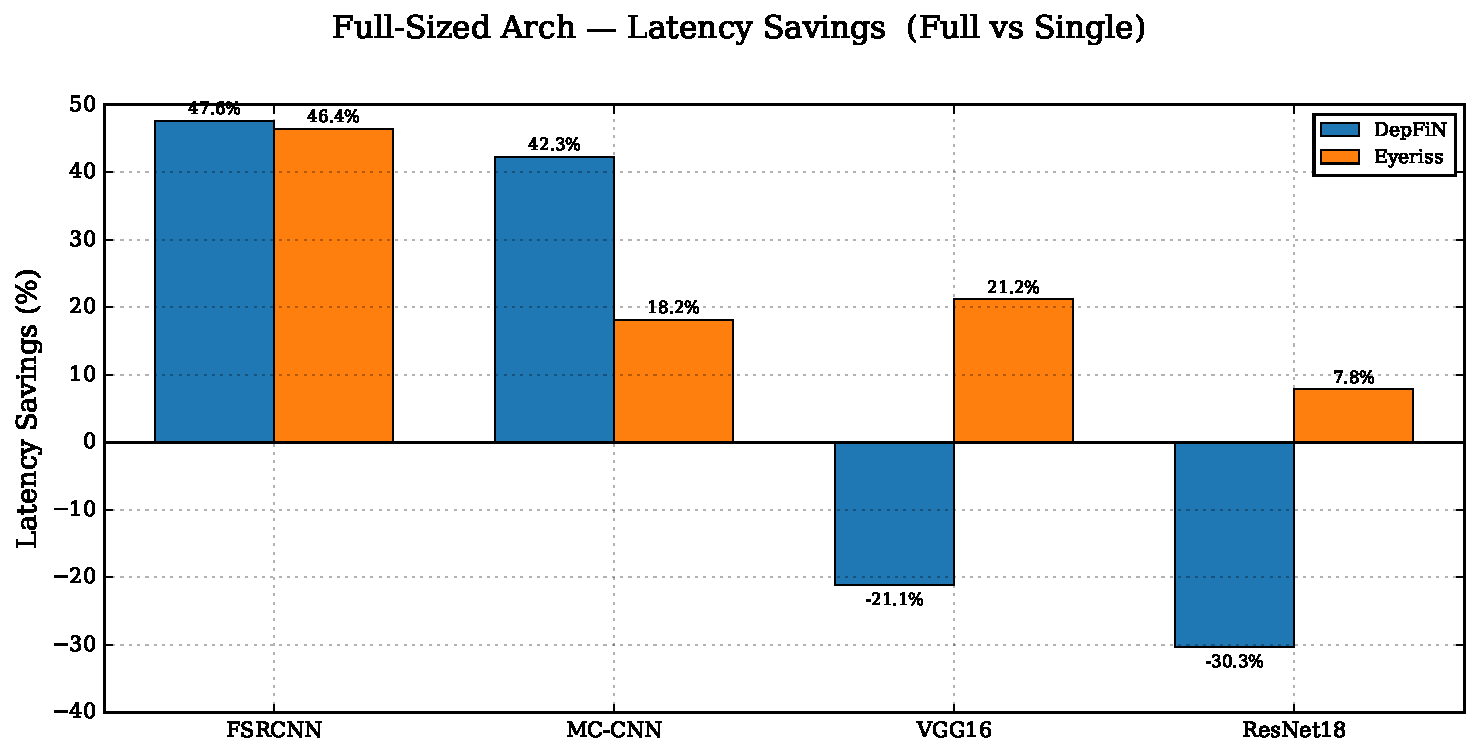
\includegraphics[width=0.75\textwidth]{plots/fusion_latency_savings.pdf}
  \caption{Scenario~A: Latency savings of full fusion relative
    to single-layer execution.
    Positive values indicate fusion is faster; negative values
    indicate fusion is slower.}
  \label{fig:fusion-latency-savings}
\end{figure}

% ── EDP ─────────────────────────────────────────────────────
\paragraph{Energy-Delay Product
  (Figure~\ref{fig:fusion-edp-norm}).}
The EDP combines energy and latency into a single efficiency
metric.

On \textbf{DepFiN}, full fusion is the clear EDP winner for the
activation-dominant workloads.
FSRCNN's single-layer EDP is $6.44\times$ the full-fusion value,
and MC-CNN is $2.31\times$: both energy and latency favor
fusion, so EDP amplifies the advantage.
For the weight-dominant workloads, however, the energy penalty of
the weight memory dominates.
VGG16 single-layer EDP is $0.035\times$ full and ResNet18 is
$0.073\times$ full.
Partial fusion occupies a middle ground: it captures most of the
latency benefit while avoiding the worst of the memory-inflation energy cost,
yielding normalized EDPs of $1.17$ (FSRCNN), $1.10$ (MC-CNN),
$0.23$ (VGG16), and $0.36$ (ResNet18).

On \textbf{Eyeriss}, the distributed register overhead shifts the
balance decisively against full fusion.
Not for FSRCNN, whose $45.6\%$ latency saving is comparable to
DepFiN's, has a full-fusion energy roughly equal to the
single-layer value ($1.02\times$), resulting in a single-layer
EDP of $1.75\times$ the full-fusion value, meaning full fusion
is still more efficient on EDP.
For MC-CNN, single-layer EDP is $0.52\times$ full, and for
VGG16 and ResNet18 it drops to $0.074\times$ and $0.13\times$,
respectively.
Partial fusion outperforms full fusion on EDP for every Eyeriss
workload, with values ranging from $0.41$ (VGG16) to $0.70$
(ResNet18).

\begin{figure}[htbp]
  \centering
  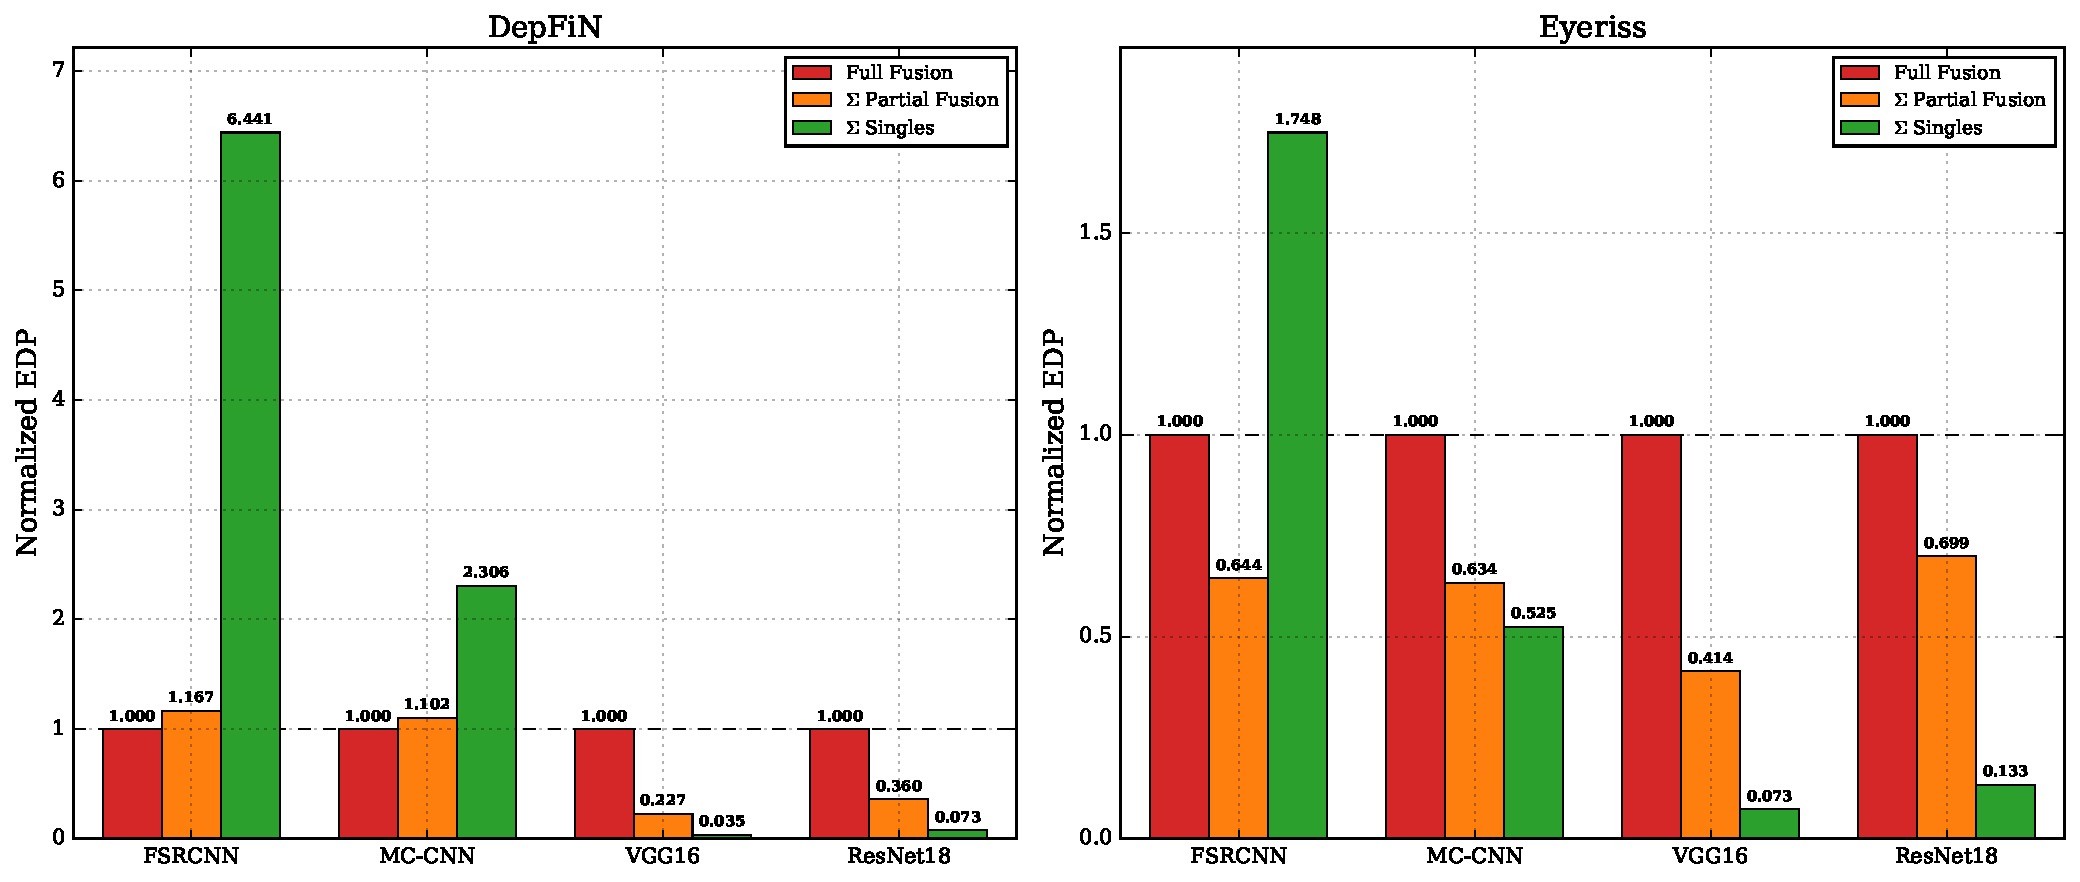
\includegraphics[width=0.95\textwidth]{plots/fusion_auto_edp_norm.pdf}
  \caption{Scenario~A: Normalized EDP (Full~Fusion\,=\,1.0).
    Bars below 1.0 indicate better efficiency than full fusion.}
  \label{fig:fusion-edp-norm}
\end{figure}

% ── DRAM Traffic ────────────────────────────────────────────
\paragraph{DRAM traffic reduction.}
\label{sec:dram-traffic}
The fundamental premise of layer fusion is the elimination of
intermediate DRAM transfers, and the data confirm that this
mechanism works as expected.
Full fusion reduces total DRAM traffic (reads + writes) by
$94.8\%$ for FSRCNN, $85.3\%$ for MC-CNN, $59.9\%$ for VGG16,
and $25.1\%$ for ResNet18, relative to single-layer execution.
These numbers are identical across the two architectures because
the DRAM access pattern depends on the tiling of the mapping, and we are trying the
same for the tile size for both the architecture for fairness of evaluation.

The reduction is largest for the activation-dominant workloads
because their intermediate activations comprise the overwhelming
majority of total DRAM traffic in single-layer mode.
For the weight-dominant workloads, weights dominate the transfer
volume, and since weights are loaded from DRAM regardless of
fusion, the relative saving is smaller.

% ── Considerations ────────────────────────────────────────────
\paragraph{Considerations.}
Full fusion achieves the elimination of
inter-layer DRAM traffic, delivering reductions of
$25$--$95\%$ depending on the workload.
This translates into significant latency improvements for
activation-dominant workloads ($42$--$48\%$ on DepFiN,
$16$--$46\%$ on Eyeriss).

The energy outcome depends on the interplay between the DRAM cost
saved and the on-chip memory overhead incurred.
At 160\,pJ\,/\,byte, full fusion is energy-beneficial on DepFiN
for activation-dominant workloads (FSRCNN, MC-CNN), where the
eliminated DRAM traffic is large and the feature memory growth is
modest.
On Eyeriss, the replicated register architecture inflates the
on-chip energy to the point where full fusion is
energy-neutral at best (FSRCNN) and energy-adverse for all other
workloads.
For weight-dominant workloads (VGG16, ResNet18), full fusion is
energy-adverse on both architectures because the massive weight
memories required for fusion drive per-access energy far above
the DRAM savings.

Partial fusion emerges as a robust compromise: it captures nearly
all of the latency benefit of full fusion while incurring a
fraction of the energy penalty, because each fused group requires
only a small memory expansion.
On EDP, full fusion wins decisively on DepFiN for the
activation-dominant workloads and marginally on Eyeriss for
FSRCNN; for all other cases, partial fusion or single-layer
execution is preferable.
The implication is that the optimal fusion strategy is
workload-dependent and architecture-dependent: activation-dominant
workloads on architectures with shared on-chip memories (DepFiN)
benefit most from aggressive fusion, while weight-dominant
workloads and architectures with replicated per-PE storage
(Eyeriss) favor partial or no fusion.